% Options for packages loaded elsewhere
\PassOptionsToPackage{unicode}{hyperref}
\PassOptionsToPackage{hyphens}{url}
\documentclass[
]{article}
\usepackage{xcolor}
\usepackage[margin=1in]{geometry}
\usepackage{amsmath,amssymb}
\setcounter{secnumdepth}{-\maxdimen} % remove section numbering
\usepackage{iftex}
\ifPDFTeX
  \usepackage[T1]{fontenc}
  \usepackage[utf8]{inputenc}
  \usepackage{textcomp} % provide euro and other symbols
\else % if luatex or xetex
  \usepackage{unicode-math} % this also loads fontspec
  \defaultfontfeatures{Scale=MatchLowercase}
  \defaultfontfeatures[\rmfamily]{Ligatures=TeX,Scale=1}
\fi
\usepackage{lmodern}
\ifPDFTeX\else
  % xetex/luatex font selection
\fi
% Use upquote if available, for straight quotes in verbatim environments
\IfFileExists{upquote.sty}{\usepackage{upquote}}{}
\IfFileExists{microtype.sty}{% use microtype if available
  \usepackage[]{microtype}
  \UseMicrotypeSet[protrusion]{basicmath} % disable protrusion for tt fonts
}{}
\makeatletter
\@ifundefined{KOMAClassName}{% if non-KOMA class
  \IfFileExists{parskip.sty}{%
    \usepackage{parskip}
  }{% else
    \setlength{\parindent}{0pt}
    \setlength{\parskip}{6pt plus 2pt minus 1pt}}
}{% if KOMA class
  \KOMAoptions{parskip=half}}
\makeatother
\usepackage{color}
\usepackage{fancyvrb}
\newcommand{\VerbBar}{|}
\newcommand{\VERB}{\Verb[commandchars=\\\{\}]}
\DefineVerbatimEnvironment{Highlighting}{Verbatim}{commandchars=\\\{\}}
% Add ',fontsize=\small' for more characters per line
\usepackage{framed}
\definecolor{shadecolor}{RGB}{248,248,248}
\newenvironment{Shaded}{\begin{snugshade}}{\end{snugshade}}
\newcommand{\AlertTok}[1]{\textcolor[rgb]{0.94,0.16,0.16}{#1}}
\newcommand{\AnnotationTok}[1]{\textcolor[rgb]{0.56,0.35,0.01}{\textbf{\textit{#1}}}}
\newcommand{\AttributeTok}[1]{\textcolor[rgb]{0.13,0.29,0.53}{#1}}
\newcommand{\BaseNTok}[1]{\textcolor[rgb]{0.00,0.00,0.81}{#1}}
\newcommand{\BuiltInTok}[1]{#1}
\newcommand{\CharTok}[1]{\textcolor[rgb]{0.31,0.60,0.02}{#1}}
\newcommand{\CommentTok}[1]{\textcolor[rgb]{0.56,0.35,0.01}{\textit{#1}}}
\newcommand{\CommentVarTok}[1]{\textcolor[rgb]{0.56,0.35,0.01}{\textbf{\textit{#1}}}}
\newcommand{\ConstantTok}[1]{\textcolor[rgb]{0.56,0.35,0.01}{#1}}
\newcommand{\ControlFlowTok}[1]{\textcolor[rgb]{0.13,0.29,0.53}{\textbf{#1}}}
\newcommand{\DataTypeTok}[1]{\textcolor[rgb]{0.13,0.29,0.53}{#1}}
\newcommand{\DecValTok}[1]{\textcolor[rgb]{0.00,0.00,0.81}{#1}}
\newcommand{\DocumentationTok}[1]{\textcolor[rgb]{0.56,0.35,0.01}{\textbf{\textit{#1}}}}
\newcommand{\ErrorTok}[1]{\textcolor[rgb]{0.64,0.00,0.00}{\textbf{#1}}}
\newcommand{\ExtensionTok}[1]{#1}
\newcommand{\FloatTok}[1]{\textcolor[rgb]{0.00,0.00,0.81}{#1}}
\newcommand{\FunctionTok}[1]{\textcolor[rgb]{0.13,0.29,0.53}{\textbf{#1}}}
\newcommand{\ImportTok}[1]{#1}
\newcommand{\InformationTok}[1]{\textcolor[rgb]{0.56,0.35,0.01}{\textbf{\textit{#1}}}}
\newcommand{\KeywordTok}[1]{\textcolor[rgb]{0.13,0.29,0.53}{\textbf{#1}}}
\newcommand{\NormalTok}[1]{#1}
\newcommand{\OperatorTok}[1]{\textcolor[rgb]{0.81,0.36,0.00}{\textbf{#1}}}
\newcommand{\OtherTok}[1]{\textcolor[rgb]{0.56,0.35,0.01}{#1}}
\newcommand{\PreprocessorTok}[1]{\textcolor[rgb]{0.56,0.35,0.01}{\textit{#1}}}
\newcommand{\RegionMarkerTok}[1]{#1}
\newcommand{\SpecialCharTok}[1]{\textcolor[rgb]{0.81,0.36,0.00}{\textbf{#1}}}
\newcommand{\SpecialStringTok}[1]{\textcolor[rgb]{0.31,0.60,0.02}{#1}}
\newcommand{\StringTok}[1]{\textcolor[rgb]{0.31,0.60,0.02}{#1}}
\newcommand{\VariableTok}[1]{\textcolor[rgb]{0.00,0.00,0.00}{#1}}
\newcommand{\VerbatimStringTok}[1]{\textcolor[rgb]{0.31,0.60,0.02}{#1}}
\newcommand{\WarningTok}[1]{\textcolor[rgb]{0.56,0.35,0.01}{\textbf{\textit{#1}}}}
\usepackage{graphicx}
\makeatletter
\newsavebox\pandoc@box
\newcommand*\pandocbounded[1]{% scales image to fit in text height/width
  \sbox\pandoc@box{#1}%
  \Gscale@div\@tempa{\textheight}{\dimexpr\ht\pandoc@box+\dp\pandoc@box\relax}%
  \Gscale@div\@tempb{\linewidth}{\wd\pandoc@box}%
  \ifdim\@tempb\p@<\@tempa\p@\let\@tempa\@tempb\fi% select the smaller of both
  \ifdim\@tempa\p@<\p@\scalebox{\@tempa}{\usebox\pandoc@box}%
  \else\usebox{\pandoc@box}%
  \fi%
}
% Set default figure placement to htbp
\def\fps@figure{htbp}
\makeatother
\setlength{\emergencystretch}{3em} % prevent overfull lines
\providecommand{\tightlist}{%
  \setlength{\itemsep}{0pt}\setlength{\parskip}{0pt}}
\usepackage{graphicx}
\usepackage{float}
\usepackage{tikz}
\usepackage{xcolor}
\usepackage{colortbl}
\usepackage{booktabs}
\usepackage{array}
\usepackage{bookmark}
\IfFileExists{xurl.sty}{\usepackage{xurl}}{} % add URL line breaks if available
\urlstyle{same}
\hypersetup{
  hidelinks,
  pdfcreator={LaTeX via pandoc}}

\author{}
\date{\vspace{-2.5em}}

\begin{document}

\begin{Shaded}
\begin{Highlighting}[]
\FunctionTok{options}\NormalTok{(}\AttributeTok{OutDec =} \StringTok{"."}\NormalTok{)  }\CommentTok{\# Asegurar punto decimal en este chunk}

\CommentTok{\# Función para generar datos aleatorios del problema}
\NormalTok{generar\_datos }\OtherTok{\textless{}{-}} \ControlFlowTok{function}\NormalTok{() \{}
  \CommentTok{\# Aleatorización de sabores de tortas (4 sabores diferentes)}
\NormalTok{  sabores\_disponibles }\OtherTok{\textless{}{-}} \FunctionTok{list}\NormalTok{(}
    \FunctionTok{c}\NormalTok{(}\StringTok{"Nuez"}\NormalTok{, }\StringTok{"Almendra"}\NormalTok{, }\StringTok{"Chocolate"}\NormalTok{, }\StringTok{"Naranja"}\NormalTok{),}
    \FunctionTok{c}\NormalTok{(}\StringTok{"Vainilla"}\NormalTok{, }\StringTok{"Fresa"}\NormalTok{, }\StringTok{"Limón"}\NormalTok{, }\StringTok{"Coco"}\NormalTok{),}
    \FunctionTok{c}\NormalTok{(}\StringTok{"Manzana"}\NormalTok{, }\StringTok{"Durazno"}\NormalTok{, }\StringTok{"Mora"}\NormalTok{, }\StringTok{"Maracuyá"}\NormalTok{),}
    \FunctionTok{c}\NormalTok{(}\StringTok{"Café"}\NormalTok{, }\StringTok{"Caramelo"}\NormalTok{, }\StringTok{"Miel"}\NormalTok{, }\StringTok{"Canela"}\NormalTok{),}
    \FunctionTok{c}\NormalTok{(}\StringTok{"Piña"}\NormalTok{, }\StringTok{"Banano"}\NormalTok{, }\StringTok{"Uva"}\NormalTok{, }\StringTok{"Cereza"}\NormalTok{)}
\NormalTok{  )}
\NormalTok{  sabores }\OtherTok{\textless{}{-}} \FunctionTok{sample}\NormalTok{(sabores\_disponibles, }\DecValTok{1}\NormalTok{)[[}\DecValTok{1}\NormalTok{]]}
  
  \CommentTok{\# Generar números de clientes que prefieren cada sabor (rango realista)}
\NormalTok{  preferencias }\OtherTok{\textless{}{-}} \FunctionTok{sample}\NormalTok{(}\DecValTok{120}\SpecialCharTok{:}\DecValTok{200}\NormalTok{, }\DecValTok{4}\NormalTok{, }\AttributeTok{replace =} \ConstantTok{TRUE}\NormalTok{)}
  \FunctionTok{names}\NormalTok{(preferencias) }\OtherTok{\textless{}{-}}\NormalTok{ sabores}
  
  \CommentTok{\# Ordenar para identificar los 2 más preferidos}
\NormalTok{  preferencias\_ordenadas }\OtherTok{\textless{}{-}} \FunctionTok{sort}\NormalTok{(preferencias, }\AttributeTok{decreasing =} \ConstantTok{TRUE}\NormalTok{)}
\NormalTok{  sabores\_mas\_preferidos }\OtherTok{\textless{}{-}} \FunctionTok{names}\NormalTok{(preferencias\_ordenadas)[}\DecValTok{1}\SpecialCharTok{:}\DecValTok{2}\NormalTok{]}
  
  \CommentTok{\# Aleatorización de días de la semana y ventas}
\NormalTok{  dias\_semana }\OtherTok{\textless{}{-}} \FunctionTok{c}\NormalTok{(}\StringTok{"Lunes"}\NormalTok{, }\StringTok{"Martes"}\NormalTok{, }\StringTok{"Miércoles"}\NormalTok{, }\StringTok{"Jueves"}\NormalTok{, }\StringTok{"Viernes"}\NormalTok{, }\StringTok{"Sábado"}\NormalTok{, }\StringTok{"Domingo"}\NormalTok{)}

  \CommentTok{\# Generar 7 valores únicos de ventas para asegurar que cada barra}
  \CommentTok{\# tenga altura diferente. Expandir el rango para tener suficientes}
  \CommentTok{\# valores únicos disponibles}
\NormalTok{  ventas\_por\_dia }\OtherTok{\textless{}{-}} \FunctionTok{sample}\NormalTok{(}\DecValTok{20}\SpecialCharTok{:}\DecValTok{60}\NormalTok{, }\DecValTok{7}\NormalTok{, }\AttributeTok{replace =} \ConstantTok{FALSE}\NormalTok{)  }\CommentTok{\# Valores únicos}
  \FunctionTok{names}\NormalTok{(ventas\_por\_dia) }\OtherTok{\textless{}{-}}\NormalTok{ dias\_semana}
  
  \CommentTok{\# Identificar el día con mayor número de ventas}
\NormalTok{  dia\_mayor\_ventas }\OtherTok{\textless{}{-}} \FunctionTok{names}\NormalTok{(}\FunctionTok{which.max}\NormalTok{(ventas\_por\_dia))}
  
  \CommentTok{\# ===== ESTRATEGIA AVANZADA DE GENERACIÓN DE OPCIONES =====}

  \CommentTok{\# 1. POOL DE OPCIONES CORRECTAS (3 formulaciones diferentes)}
\NormalTok{  pool\_correctas }\OtherTok{\textless{}{-}} \FunctionTok{c}\NormalTok{(}
    \FunctionTok{paste0}\NormalTok{(}\StringTok{"Se venderán el "}\NormalTok{, }\FunctionTok{tolower}\NormalTok{(dia\_mayor\_ventas),}
           \StringTok{" y los sabores serán "}\NormalTok{, }\FunctionTok{tolower}\NormalTok{(sabores\_mas\_preferidos[}\DecValTok{1}\NormalTok{]),}
           \StringTok{" y "}\NormalTok{, }\FunctionTok{tolower}\NormalTok{(sabores\_mas\_preferidos[}\DecValTok{2}\NormalTok{]), }\StringTok{"."}\NormalTok{),}
    \FunctionTok{paste0}\NormalTok{(}\StringTok{"La promoción será el "}\NormalTok{, }\FunctionTok{tolower}\NormalTok{(dia\_mayor\_ventas),}
           \StringTok{" con tortas de "}\NormalTok{, }\FunctionTok{tolower}\NormalTok{(sabores\_mas\_preferidos[}\DecValTok{1}\NormalTok{]),}
           \StringTok{" y "}\NormalTok{, }\FunctionTok{tolower}\NormalTok{(sabores\_mas\_preferidos[}\DecValTok{2}\NormalTok{]), }\StringTok{"."}\NormalTok{),}
    \FunctionTok{paste0}\NormalTok{(}\StringTok{"El día "}\NormalTok{, }\FunctionTok{tolower}\NormalTok{(dia\_mayor\_ventas),}
           \StringTok{" se ofrecerán sabores "}\NormalTok{, }\FunctionTok{tolower}\NormalTok{(sabores\_mas\_preferidos[}\DecValTok{1}\NormalTok{]),}
           \StringTok{" y "}\NormalTok{, }\FunctionTok{tolower}\NormalTok{(sabores\_mas\_preferidos[}\DecValTok{2}\NormalTok{]), }\StringTok{"."}\NormalTok{)}
\NormalTok{  )}

  \CommentTok{\# Seleccionar aleatoriamente 1 opción correcta del pool}
\NormalTok{  respuesta\_correcta }\OtherTok{\textless{}{-}} \FunctionTok{sample}\NormalTok{(pool\_correctas, }\DecValTok{1}\NormalTok{)}

  \CommentTok{\# 2. POOL DE DISTRACTORES PEDAGÓGICOS (6 distractores específicos)}
\NormalTok{  otros\_dias }\OtherTok{\textless{}{-}}\NormalTok{ dias\_semana[dias\_semana }\SpecialCharTok{!=}\NormalTok{ dia\_mayor\_ventas]}
\NormalTok{  otros\_sabores }\OtherTok{\textless{}{-}}\NormalTok{ sabores[}\SpecialCharTok{!}\NormalTok{sabores }\SpecialCharTok{\%in\%}\NormalTok{ sabores\_mas\_preferidos]}

  \CommentTok{\# Distractores tipo 1: Día correcto, sabores incorrectos (2 opciones)}
\NormalTok{  distractores\_tipo1 }\OtherTok{\textless{}{-}} \FunctionTok{c}\NormalTok{(}
    \FunctionTok{paste0}\NormalTok{(}\StringTok{"Se venderán el "}\NormalTok{, }\FunctionTok{tolower}\NormalTok{(dia\_mayor\_ventas),}
           \StringTok{" y los sabores serán "}\NormalTok{, }\FunctionTok{tolower}\NormalTok{(otros\_sabores[}\DecValTok{1}\NormalTok{]),}
           \StringTok{" y "}\NormalTok{, }\FunctionTok{tolower}\NormalTok{(otros\_sabores[}\DecValTok{2}\NormalTok{]), }\StringTok{"."}\NormalTok{),}
    \FunctionTok{paste0}\NormalTok{(}\StringTok{"La promoción será el "}\NormalTok{, }\FunctionTok{tolower}\NormalTok{(dia\_mayor\_ventas),}
           \StringTok{" con tortas de "}\NormalTok{, }\FunctionTok{tolower}\NormalTok{(otros\_sabores[}\DecValTok{2}\NormalTok{]),}
           \StringTok{" y "}\NormalTok{, }\FunctionTok{tolower}\NormalTok{(sabores\_mas\_preferidos[}\DecValTok{2}\NormalTok{]), }\StringTok{"."}\NormalTok{)}
\NormalTok{  )}

  \CommentTok{\# Distractores tipo 2: Sabores correctos, día incorrecto (2 opciones)}
\NormalTok{  dias\_distractores }\OtherTok{\textless{}{-}} \FunctionTok{sample}\NormalTok{(otros\_dias, }\DecValTok{2}\NormalTok{)}
\NormalTok{  distractores\_tipo2 }\OtherTok{\textless{}{-}} \FunctionTok{c}\NormalTok{(}
    \FunctionTok{paste0}\NormalTok{(}\StringTok{"Se venderán el "}\NormalTok{, }\FunctionTok{tolower}\NormalTok{(dias\_distractores[}\DecValTok{1}\NormalTok{]),}
           \StringTok{" y los sabores serán "}\NormalTok{, }\FunctionTok{tolower}\NormalTok{(sabores\_mas\_preferidos[}\DecValTok{1}\NormalTok{]),}
           \StringTok{" y "}\NormalTok{, }\FunctionTok{tolower}\NormalTok{(sabores\_mas\_preferidos[}\DecValTok{2}\NormalTok{]), }\StringTok{"."}\NormalTok{),}
    \FunctionTok{paste0}\NormalTok{(}\StringTok{"El día "}\NormalTok{, }\FunctionTok{tolower}\NormalTok{(dias\_distractores[}\DecValTok{2}\NormalTok{]),}
           \StringTok{" se ofrecerán sabores "}\NormalTok{, }\FunctionTok{tolower}\NormalTok{(sabores\_mas\_preferidos[}\DecValTok{1}\NormalTok{]),}
           \StringTok{" y "}\NormalTok{, }\FunctionTok{tolower}\NormalTok{(sabores\_mas\_preferidos[}\DecValTok{2}\NormalTok{]), }\StringTok{"."}\NormalTok{)}
\NormalTok{  )}

  \CommentTok{\# Distractores tipo 3: Ambos elementos incorrectos pero plausibles (2 opciones)}
\NormalTok{  dias\_distractores\_extra }\OtherTok{\textless{}{-}} \FunctionTok{sample}\NormalTok{(otros\_dias[}\SpecialCharTok{!}\NormalTok{otros\_dias }\SpecialCharTok{\%in\%}\NormalTok{ dias\_distractores], }\DecValTok{2}\NormalTok{)}
\NormalTok{  distractores\_tipo3 }\OtherTok{\textless{}{-}} \FunctionTok{c}\NormalTok{(}
    \FunctionTok{paste0}\NormalTok{(}\StringTok{"Se venderán el "}\NormalTok{, }\FunctionTok{tolower}\NormalTok{(dias\_distractores\_extra[}\DecValTok{1}\NormalTok{]),}
           \StringTok{" y los sabores serán "}\NormalTok{, }\FunctionTok{tolower}\NormalTok{(otros\_sabores[}\DecValTok{1}\NormalTok{]),}
           \StringTok{" y "}\NormalTok{, }\FunctionTok{tolower}\NormalTok{(sabores\_mas\_preferidos[}\DecValTok{1}\NormalTok{]), }\StringTok{"."}\NormalTok{),}
    \FunctionTok{paste0}\NormalTok{(}\StringTok{"La promoción será el "}\NormalTok{, }\FunctionTok{tolower}\NormalTok{(dias\_distractores\_extra[}\DecValTok{2}\NormalTok{]),}
           \StringTok{" con tortas de "}\NormalTok{, }\FunctionTok{tolower}\NormalTok{(otros\_sabores[}\DecValTok{2}\NormalTok{]),}
           \StringTok{" y "}\NormalTok{, }\FunctionTok{tolower}\NormalTok{(otros\_sabores[}\DecValTok{1}\NormalTok{]), }\StringTok{"."}\NormalTok{)}
\NormalTok{  )}

  \CommentTok{\# Pool completo de distractores}
\NormalTok{  pool\_distractores }\OtherTok{\textless{}{-}} \FunctionTok{c}\NormalTok{(distractores\_tipo1, distractores\_tipo2, distractores\_tipo3)}

  \CommentTok{\# 3. VALIDACIÓN DE UNICIDAD Y SELECCIÓN}
  \CommentTok{\# Función para calcular similitud textual}
\NormalTok{  calcular\_similitud }\OtherTok{\textless{}{-}} \ControlFlowTok{function}\NormalTok{(texto1, texto2) \{}
\NormalTok{    palabras1 }\OtherTok{\textless{}{-}} \FunctionTok{strsplit}\NormalTok{(}\FunctionTok{tolower}\NormalTok{(texto1), }\StringTok{"}\SpecialCharTok{\textbackslash{}\textbackslash{}}\StringTok{W+"}\NormalTok{)[[}\DecValTok{1}\NormalTok{]]}
\NormalTok{    palabras2 }\OtherTok{\textless{}{-}} \FunctionTok{strsplit}\NormalTok{(}\FunctionTok{tolower}\NormalTok{(texto2), }\StringTok{"}\SpecialCharTok{\textbackslash{}\textbackslash{}}\StringTok{W+"}\NormalTok{)[[}\DecValTok{1}\NormalTok{]]}
\NormalTok{    interseccion }\OtherTok{\textless{}{-}} \FunctionTok{length}\NormalTok{(}\FunctionTok{intersect}\NormalTok{(palabras1, palabras2))}
\NormalTok{    union }\OtherTok{\textless{}{-}} \FunctionTok{length}\NormalTok{(}\FunctionTok{union}\NormalTok{(palabras1, palabras2))}
    \FunctionTok{return}\NormalTok{(interseccion }\SpecialCharTok{/}\NormalTok{ union)}
\NormalTok{  \}}

  \CommentTok{\# Seleccionar 3 distractores únicos}
\NormalTok{  distractores\_seleccionados }\OtherTok{\textless{}{-}} \FunctionTok{c}\NormalTok{()}
\NormalTok{  tipos\_seleccionados }\OtherTok{\textless{}{-}} \FunctionTok{c}\NormalTok{()  }\CommentTok{\# Para trazabilidad}
\NormalTok{  intentos }\OtherTok{\textless{}{-}} \DecValTok{0}
\NormalTok{  max\_intentos }\OtherTok{\textless{}{-}} \DecValTok{50}  \CommentTok{\# Reducido para eficiencia}

  \ControlFlowTok{while}\NormalTok{(}\FunctionTok{length}\NormalTok{(distractores\_seleccionados) }\SpecialCharTok{\textless{}} \DecValTok{3} \SpecialCharTok{\&\&}\NormalTok{ intentos }\SpecialCharTok{\textless{}}\NormalTok{ max\_intentos) \{}
\NormalTok{    intentos }\OtherTok{\textless{}{-}}\NormalTok{ intentos }\SpecialCharTok{+} \DecValTok{1}

    \CommentTok{\# Seleccionar un distractor aleatorio}
\NormalTok{    candidato\_idx }\OtherTok{\textless{}{-}} \FunctionTok{sample}\NormalTok{(}\DecValTok{1}\SpecialCharTok{:}\FunctionTok{length}\NormalTok{(pool\_distractores), }\DecValTok{1}\NormalTok{)}
\NormalTok{    candidato }\OtherTok{\textless{}{-}}\NormalTok{ pool\_distractores[candidato\_idx]}

    \CommentTok{\# Determinar tipo de distractor para trazabilidad}
    \ControlFlowTok{if}\NormalTok{(candidato\_idx }\SpecialCharTok{\textless{}=} \DecValTok{2}\NormalTok{) \{}
\NormalTok{      tipo\_candidato }\OtherTok{\textless{}{-}} \StringTok{"dia\_correcto\_sabores\_incorrectos"}
\NormalTok{    \} }\ControlFlowTok{else} \ControlFlowTok{if}\NormalTok{(candidato\_idx }\SpecialCharTok{\textless{}=} \DecValTok{4}\NormalTok{) \{}
\NormalTok{      tipo\_candidato }\OtherTok{\textless{}{-}} \StringTok{"sabores\_correctos\_dia\_incorrecto"}
\NormalTok{    \} }\ControlFlowTok{else}\NormalTok{ \{}
\NormalTok{      tipo\_candidato }\OtherTok{\textless{}{-}} \StringTok{"ambos\_incorrectos\_plausibles"}
\NormalTok{    \}}

    \CommentTok{\# Verificar unicidad con respuesta correcta}
\NormalTok{    similitud\_correcta }\OtherTok{\textless{}{-}} \FunctionTok{calcular\_similitud}\NormalTok{(candidato, respuesta\_correcta)}

    \CommentTok{\# Verificar unicidad con distractores ya seleccionados}
\NormalTok{    es\_unico }\OtherTok{\textless{}{-}} \ConstantTok{TRUE}
    \ControlFlowTok{if}\NormalTok{(}\FunctionTok{length}\NormalTok{(distractores\_seleccionados) }\SpecialCharTok{\textgreater{}} \DecValTok{0}\NormalTok{) \{}
      \ControlFlowTok{for}\NormalTok{(distractor\_existente }\ControlFlowTok{in}\NormalTok{ distractores\_seleccionados) \{}
\NormalTok{        similitud\_distractor }\OtherTok{\textless{}{-}} \FunctionTok{calcular\_similitud}\NormalTok{(candidato, distractor\_existente)}
        \ControlFlowTok{if}\NormalTok{(similitud\_distractor }\SpecialCharTok{\textgreater{}} \FloatTok{0.4}\NormalTok{) \{  }\CommentTok{\# Umbral más realista del 60\% de diferencia}
\NormalTok{          es\_unico }\OtherTok{\textless{}{-}} \ConstantTok{FALSE}
          \ControlFlowTok{break}
\NormalTok{        \}}
\NormalTok{      \}}
\NormalTok{    \}}

    \CommentTok{\# Agregar si es único y suficientemente diferente}
    \ControlFlowTok{if}\NormalTok{(es\_unico }\SpecialCharTok{\&\&}\NormalTok{ similitud\_correcta }\SpecialCharTok{\textless{}} \FloatTok{0.4}\NormalTok{) \{}
\NormalTok{      distractores\_seleccionados }\OtherTok{\textless{}{-}} \FunctionTok{c}\NormalTok{(distractores\_seleccionados, candidato)}
\NormalTok{      tipos\_seleccionados }\OtherTok{\textless{}{-}} \FunctionTok{c}\NormalTok{(tipos\_seleccionados, tipo\_candidato)}

      \CommentTok{\# Remover del pool para evitar reselección}
\NormalTok{      pool\_distractores }\OtherTok{\textless{}{-}}\NormalTok{ pool\_distractores[}\SpecialCharTok{{-}}\NormalTok{candidato\_idx]}
\NormalTok{    \}}
\NormalTok{  \}}

  \CommentTok{\# Si no se pudieron generar 3 distractores únicos, usar los primeros 3 del pool}
  \ControlFlowTok{if}\NormalTok{(}\FunctionTok{length}\NormalTok{(distractores\_seleccionados) }\SpecialCharTok{\textless{}} \DecValTok{3}\NormalTok{) \{}
\NormalTok{    distractores\_seleccionados }\OtherTok{\textless{}{-}}\NormalTok{ pool\_distractores[}\DecValTok{1}\SpecialCharTok{:}\DecValTok{3}\NormalTok{]}
\NormalTok{    tipos\_seleccionados }\OtherTok{\textless{}{-}} \FunctionTok{c}\NormalTok{(}\StringTok{"dia\_correcto\_sabores\_incorrectos"}\NormalTok{,}
                           \StringTok{"sabores\_correctos\_dia\_incorrecto"}\NormalTok{,}
                           \StringTok{"ambos\_incorrectos\_plausibles"}\NormalTok{)}
\NormalTok{  \}}

  \CommentTok{\# 4. ALEATORIZACIÓN Y POSICIONAMIENTO}
\NormalTok{  todas\_opciones }\OtherTok{\textless{}{-}} \FunctionTok{c}\NormalTok{(respuesta\_correcta, distractores\_seleccionados)}
\NormalTok{  orden\_opciones }\OtherTok{\textless{}{-}} \FunctionTok{sample}\NormalTok{(}\DecValTok{1}\SpecialCharTok{:}\DecValTok{4}\NormalTok{)}
\NormalTok{  opciones\_mezcladas }\OtherTok{\textless{}{-}}\NormalTok{ todas\_opciones[orden\_opciones]}
\NormalTok{  posicion\_correcta }\OtherTok{\textless{}{-}} \FunctionTok{which}\NormalTok{(orden\_opciones }\SpecialCharTok{==} \DecValTok{1}\NormalTok{)}

  \CommentTok{\# 5. DOCUMENTACIÓN Y TRAZABILIDAD}
  \CommentTok{\# Crear mapeo de tipos de distractores para cada posición}
\NormalTok{  tipos\_opciones }\OtherTok{\textless{}{-}} \FunctionTok{c}\NormalTok{(}\StringTok{"respuesta\_correcta"}\NormalTok{, tipos\_seleccionados)}
\NormalTok{  tipos\_mezclados }\OtherTok{\textless{}{-}}\NormalTok{ tipos\_opciones[orden\_opciones]}
  
  \FunctionTok{return}\NormalTok{(}\FunctionTok{list}\NormalTok{(}
    \AttributeTok{sabores =}\NormalTok{ sabores,}
    \AttributeTok{preferencias =}\NormalTok{ preferencias,}
    \AttributeTok{sabores\_mas\_preferidos =}\NormalTok{ sabores\_mas\_preferidos,}
    \AttributeTok{dias\_semana =}\NormalTok{ dias\_semana,}
    \AttributeTok{ventas\_por\_dia =}\NormalTok{ ventas\_por\_dia,}
    \AttributeTok{dia\_mayor\_ventas =}\NormalTok{ dia\_mayor\_ventas,}
    \AttributeTok{opciones =}\NormalTok{ opciones\_mezcladas,}
    \AttributeTok{respuesta\_correcta =}\NormalTok{ respuesta\_correcta,}
    \AttributeTok{posicion\_correcta =}\NormalTok{ posicion\_correcta,}
    \CommentTok{\# Información de trazabilidad para debugging y análisis pedagógico}
    \AttributeTok{tipos\_opciones =}\NormalTok{ tipos\_mezclados,}
    \AttributeTok{pool\_correcta\_usada =} \FunctionTok{which}\NormalTok{(pool\_correctas }\SpecialCharTok{==}\NormalTok{ respuesta\_correcta),}
    \AttributeTok{distractores\_tipos =}\NormalTok{ tipos\_seleccionados,}
    \AttributeTok{validacion\_unicidad =} \FunctionTok{list}\NormalTok{(}
      \AttributeTok{intentos\_realizados =}\NormalTok{ intentos,}
      \AttributeTok{distractores\_generados =} \FunctionTok{length}\NormalTok{(distractores\_seleccionados)}
\NormalTok{    )}
\NormalTok{  ))}
\NormalTok{\}}

\CommentTok{\# Generar datos para este ejercicio}
\NormalTok{datos }\OtherTok{\textless{}{-}} \FunctionTok{generar\_datos}\NormalTok{()}
\end{Highlighting}
\end{Shaded}

\begin{Shaded}
\begin{Highlighting}[]
\CommentTok{\# Crear tabla de preferencias usando TikZ}
\NormalTok{tabla\_preferencias }\OtherTok{\textless{}{-}} \FunctionTok{paste0}\NormalTok{(}\StringTok{"}
\SpecialCharTok{\textbackslash{}\textbackslash{}}\StringTok{begin\{tikzpicture\}}
\SpecialCharTok{\textbackslash{}\textbackslash{}}\StringTok{node[inner sep=0pt] \{}
\StringTok{  }\SpecialCharTok{\textbackslash{}\textbackslash{}}\StringTok{begin\{tabular\}\{|c|c|\}}
\StringTok{    }\SpecialCharTok{\textbackslash{}\textbackslash{}}\StringTok{hline}
\StringTok{    }\SpecialCharTok{\textbackslash{}\textbackslash{}}\StringTok{textbf\{Sabor\} \& }\SpecialCharTok{\textbackslash{}\textbackslash{}}\StringTok{textbf\{Número de clientes que\} }\SpecialCharTok{\textbackslash{}\textbackslash{}\textbackslash{}\textbackslash{}}
\StringTok{    \& }\SpecialCharTok{\textbackslash{}\textbackslash{}}\StringTok{textbf\{prefieren el sabor\} }\SpecialCharTok{\textbackslash{}\textbackslash{}\textbackslash{}\textbackslash{}}
\StringTok{    }\SpecialCharTok{\textbackslash{}\textbackslash{}}\StringTok{hline}
\StringTok{    "}\NormalTok{, datos}\SpecialCharTok{$}\NormalTok{sabores[}\DecValTok{1}\NormalTok{], }\StringTok{" \& "}\NormalTok{, datos}\SpecialCharTok{$}\NormalTok{preferencias[datos}\SpecialCharTok{$}\NormalTok{sabores[}\DecValTok{1}\NormalTok{]], }\StringTok{" clientes }\SpecialCharTok{\textbackslash{}\textbackslash{}\textbackslash{}\textbackslash{}}
\StringTok{    }\SpecialCharTok{\textbackslash{}\textbackslash{}}\StringTok{hline}
\StringTok{    "}\NormalTok{, datos}\SpecialCharTok{$}\NormalTok{sabores[}\DecValTok{2}\NormalTok{], }\StringTok{" \& "}\NormalTok{, datos}\SpecialCharTok{$}\NormalTok{preferencias[datos}\SpecialCharTok{$}\NormalTok{sabores[}\DecValTok{2}\NormalTok{]], }\StringTok{" clientes }\SpecialCharTok{\textbackslash{}\textbackslash{}\textbackslash{}\textbackslash{}}
\StringTok{    }\SpecialCharTok{\textbackslash{}\textbackslash{}}\StringTok{hline}
\StringTok{    "}\NormalTok{, datos}\SpecialCharTok{$}\NormalTok{sabores[}\DecValTok{3}\NormalTok{], }\StringTok{" \& "}\NormalTok{, datos}\SpecialCharTok{$}\NormalTok{preferencias[datos}\SpecialCharTok{$}\NormalTok{sabores[}\DecValTok{3}\NormalTok{]], }\StringTok{" clientes }\SpecialCharTok{\textbackslash{}\textbackslash{}\textbackslash{}\textbackslash{}}
\StringTok{    }\SpecialCharTok{\textbackslash{}\textbackslash{}}\StringTok{hline}
\StringTok{    "}\NormalTok{, datos}\SpecialCharTok{$}\NormalTok{sabores[}\DecValTok{4}\NormalTok{], }\StringTok{" \& "}\NormalTok{, datos}\SpecialCharTok{$}\NormalTok{preferencias[datos}\SpecialCharTok{$}\NormalTok{sabores[}\DecValTok{4}\NormalTok{]], }\StringTok{" clientes }\SpecialCharTok{\textbackslash{}\textbackslash{}\textbackslash{}\textbackslash{}}
\StringTok{    }\SpecialCharTok{\textbackslash{}\textbackslash{}}\StringTok{hline}
\StringTok{  }\SpecialCharTok{\textbackslash{}\textbackslash{}}\StringTok{end\{tabular\}}
\StringTok{\};}
\SpecialCharTok{\textbackslash{}\textbackslash{}}\StringTok{end\{tikzpicture\}}
\StringTok{"}\NormalTok{)}

\CommentTok{\# Crear gráfico de barras usando TikZ}
\NormalTok{max\_ventas }\OtherTok{\textless{}{-}} \FunctionTok{max}\NormalTok{(datos}\SpecialCharTok{$}\NormalTok{ventas\_por\_dia)}
\NormalTok{escala\_y }\OtherTok{\textless{}{-}} \DecValTok{50} \SpecialCharTok{/}\NormalTok{ max\_ventas  }\CommentTok{\# Escalar para que la barra más alta sea 50 unidades}

\NormalTok{grafico\_barras }\OtherTok{\textless{}{-}} \FunctionTok{paste0}\NormalTok{(}\StringTok{"}
\SpecialCharTok{\textbackslash{}\textbackslash{}}\StringTok{begin\{tikzpicture\}[scale=0.8]}
\StringTok{  }\SpecialCharTok{\textbackslash{}\textbackslash{}}\StringTok{draw[{-}\textgreater{}] (0,0) {-}{-} (8,0) node[right] \{Día\};}
\StringTok{  }\SpecialCharTok{\textbackslash{}\textbackslash{}}\StringTok{draw[{-}\textgreater{}] (0,0) {-}{-} (0,6) node[above] \{Tortas vendidas\};}
\StringTok{  }
\StringTok{  \% Etiquetas del eje Y}
\StringTok{  }\SpecialCharTok{\textbackslash{}\textbackslash{}}\StringTok{foreach }\SpecialCharTok{\textbackslash{}\textbackslash{}}\StringTok{y in \{0,10,20,30,40,50\}}
\StringTok{    }\SpecialCharTok{\textbackslash{}\textbackslash{}}\StringTok{draw ({-}0.1,}\SpecialCharTok{\textbackslash{}\textbackslash{}}\StringTok{y/10) {-}{-} (0.1,}\SpecialCharTok{\textbackslash{}\textbackslash{}}\StringTok{y/10) node[left] \{}\SpecialCharTok{\textbackslash{}\textbackslash{}}\StringTok{y\};}
\StringTok{  }
\StringTok{  \% Barras y etiquetas}
\StringTok{  }\SpecialCharTok{\textbackslash{}\textbackslash{}}\StringTok{draw[fill=lightgray] (0.5,0) rectangle (1,"}\NormalTok{, datos}\SpecialCharTok{$}\NormalTok{ventas\_por\_dia[}\DecValTok{1}\NormalTok{] }\SpecialCharTok{*}\NormalTok{ escala\_y }\SpecialCharTok{/} \DecValTok{10}\NormalTok{, }\StringTok{") node[above] \{"}\NormalTok{, datos}\SpecialCharTok{$}\NormalTok{ventas\_por\_dia[}\DecValTok{1}\NormalTok{], }\StringTok{"\};}
\StringTok{  }\SpecialCharTok{\textbackslash{}\textbackslash{}}\StringTok{draw[fill=lightgray] (1.5,0) rectangle (2,"}\NormalTok{, datos}\SpecialCharTok{$}\NormalTok{ventas\_por\_dia[}\DecValTok{2}\NormalTok{] }\SpecialCharTok{*}\NormalTok{ escala\_y }\SpecialCharTok{/} \DecValTok{10}\NormalTok{, }\StringTok{") node[above] \{"}\NormalTok{, datos}\SpecialCharTok{$}\NormalTok{ventas\_por\_dia[}\DecValTok{2}\NormalTok{], }\StringTok{"\};}
\StringTok{  }\SpecialCharTok{\textbackslash{}\textbackslash{}}\StringTok{draw[fill=lightgray] (2.5,0) rectangle (3,"}\NormalTok{, datos}\SpecialCharTok{$}\NormalTok{ventas\_por\_dia[}\DecValTok{3}\NormalTok{] }\SpecialCharTok{*}\NormalTok{ escala\_y }\SpecialCharTok{/} \DecValTok{10}\NormalTok{, }\StringTok{") node[above] \{"}\NormalTok{, datos}\SpecialCharTok{$}\NormalTok{ventas\_por\_dia[}\DecValTok{3}\NormalTok{], }\StringTok{"\};}
\StringTok{  }\SpecialCharTok{\textbackslash{}\textbackslash{}}\StringTok{draw[fill=lightgray] (3.5,0) rectangle (4,"}\NormalTok{, datos}\SpecialCharTok{$}\NormalTok{ventas\_por\_dia[}\DecValTok{4}\NormalTok{] }\SpecialCharTok{*}\NormalTok{ escala\_y }\SpecialCharTok{/} \DecValTok{10}\NormalTok{, }\StringTok{") node[above] \{"}\NormalTok{, datos}\SpecialCharTok{$}\NormalTok{ventas\_por\_dia[}\DecValTok{4}\NormalTok{], }\StringTok{"\};}
\StringTok{  }\SpecialCharTok{\textbackslash{}\textbackslash{}}\StringTok{draw[fill=lightgray] (4.5,0) rectangle (5,"}\NormalTok{, datos}\SpecialCharTok{$}\NormalTok{ventas\_por\_dia[}\DecValTok{5}\NormalTok{] }\SpecialCharTok{*}\NormalTok{ escala\_y }\SpecialCharTok{/} \DecValTok{10}\NormalTok{, }\StringTok{") node[above] \{"}\NormalTok{, datos}\SpecialCharTok{$}\NormalTok{ventas\_por\_dia[}\DecValTok{5}\NormalTok{], }\StringTok{"\};}
\StringTok{  }\SpecialCharTok{\textbackslash{}\textbackslash{}}\StringTok{draw[fill=lightgray] (5.5,0) rectangle (6,"}\NormalTok{, datos}\SpecialCharTok{$}\NormalTok{ventas\_por\_dia[}\DecValTok{6}\NormalTok{] }\SpecialCharTok{*}\NormalTok{ escala\_y }\SpecialCharTok{/} \DecValTok{10}\NormalTok{, }\StringTok{") node[above] \{"}\NormalTok{, datos}\SpecialCharTok{$}\NormalTok{ventas\_por\_dia[}\DecValTok{6}\NormalTok{], }\StringTok{"\};}
\StringTok{  }\SpecialCharTok{\textbackslash{}\textbackslash{}}\StringTok{draw[fill=lightgray] (6.5,0) rectangle (7,"}\NormalTok{, datos}\SpecialCharTok{$}\NormalTok{ventas\_por\_dia[}\DecValTok{7}\NormalTok{] }\SpecialCharTok{*}\NormalTok{ escala\_y }\SpecialCharTok{/} \DecValTok{10}\NormalTok{, }\StringTok{") node[above] \{"}\NormalTok{, datos}\SpecialCharTok{$}\NormalTok{ventas\_por\_dia[}\DecValTok{7}\NormalTok{], }\StringTok{"\};}
\StringTok{  }
\StringTok{  \% Etiquetas del eje X}
\StringTok{  }\SpecialCharTok{\textbackslash{}\textbackslash{}}\StringTok{node[below] at (0.75,{-}0.3) \{Lun\};}
\StringTok{  }\SpecialCharTok{\textbackslash{}\textbackslash{}}\StringTok{node[below] at (1.75,{-}0.3) \{Mar\};}
\StringTok{  }\SpecialCharTok{\textbackslash{}\textbackslash{}}\StringTok{node[below] at (2.75,{-}0.3) \{Mié\};}
\StringTok{  }\SpecialCharTok{\textbackslash{}\textbackslash{}}\StringTok{node[below] at (3.75,{-}0.3) \{Jue\};}
\StringTok{  }\SpecialCharTok{\textbackslash{}\textbackslash{}}\StringTok{node[below] at (4.75,{-}0.3) \{Vie\};}
\StringTok{  }\SpecialCharTok{\textbackslash{}\textbackslash{}}\StringTok{node[below] at (5.75,{-}0.3) \{Sáb\};}
\StringTok{  }\SpecialCharTok{\textbackslash{}\textbackslash{}}\StringTok{node[below] at (6.75,{-}0.3) \{Dom\};}
\SpecialCharTok{\textbackslash{}\textbackslash{}}\StringTok{end\{tikzpicture\}}
\StringTok{"}\NormalTok{)}
\end{Highlighting}
\end{Shaded}

\section{Question}\label{question}

Una pastelería realizó una encuesta para conocer los sabores de tortas
preferidos por sus clientes. La tabla muestra los resultados de la
encuesta.

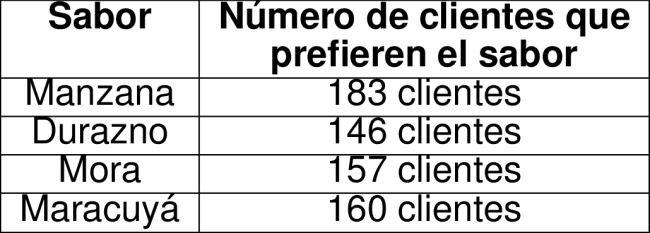
\includegraphics[width=8cm,height=\textheight,keepaspectratio]{tabla_preferencias.png}

Además, el gerente elaboró una gráfica que muestra el número de tortas
vendidas cada día de la última semana.

\textbf{Tortas vendidas durante la última semana}

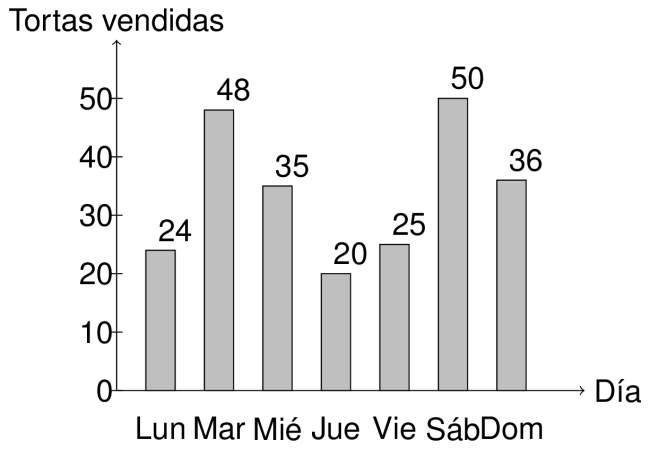
\includegraphics[width=10cm,height=\textheight,keepaspectratio]{grafico_ventas.png}

La pastelería planea realizar una promoción con tortas de los 2 sabores
preferidos por los clientes, para venderlas el día de la semana con el
mayor número de ventas. ¿Cuál día de la semana se venderán las tortas y
de qué sabores serán?

\subsection{Answerlist}\label{answerlist}

\begin{itemize}
\tightlist
\item
  Se venderán el miércoles y los sabores serán caramelo y canela.
\item
  Se venderán el jueves y los sabores serán café y caramelo.
\item
  La promoción será el sábado con tortas de caramelo y canela.
\item
  La promoción será el sábado con tortas de miel y canela.
\end{itemize}

\section{Solution}\label{solution}

Para resolver este problema, necesitamos:

\begin{enumerate}
\def\labelenumi{\arabic{enumi}.}
\tightlist
\item
  \textbf{Identificar los 2 sabores más preferidos} según la tabla de
  encuesta
\item
  \textbf{Identificar el día con mayor número de ventas} según el
  gráfico de barras
\end{enumerate}

\textbf{Análisis de la tabla de preferencias:}

\begin{itemize}
\tightlist
\item
  Caramelo : 193 clientes
\item
  Canela : 191 clientes
\item
  Miel : 182 clientes
\item
  Café : 151 clientes
\end{itemize}

Los 2 sabores más preferidos son: \textbf{Caramelo} y \textbf{Canela}.

\textbf{Análisis del gráfico de ventas:}

El día con mayor número de ventas es: ** Sábado ** con 58 tortas
vendidas.

\textbf{Respuesta:} Se venderán el sábado y los sabores serán caramelo y
canela.

\subsection{Answerlist}\label{answerlist-1}

\begin{itemize}
\tightlist
\item
  \textbf{Incorrecto.} Identifica correctamente los 2 sabores más
  preferidos, pero no selecciona el día con mayor número de ventas según
  el gráfico.
\item
  \textbf{Incorrecto.} No identifica correctamente ni el día con mayor
  número de ventas ni los 2 sabores más preferidos. Revisa
  cuidadosamente ambos datos.
\item
  \textbf{Correcto.} Identifica correctamente tanto el día con mayor
  número de ventas como los 2 sabores más preferidos según los datos
  presentados.
\item
  \textbf{Incorrecto.} Identifica correctamente el día con mayor número
  de ventas, pero no selecciona los 2 sabores más preferidos según la
  tabla de encuesta.
\end{itemize}

\section{Meta-information}\label{meta-information}

exname: pasteleria\_sabores\_ventas\_estadistica extype: schoice
exsolution: 0010 exshuffle: TRUE exsection: Estadística/Interpretación
de datos/Gráficos y tablas

\end{document}
